\chapter{Teoretický základ}
\label{2-teorie}
%co v kapitole uvedu?
V této kapitole představím Informační systém katastru nemovitostí a doplním o způsob poskytování dat z katastru nemovitostí. Text této kapitoly vychází z informací o \zk{ISKN} na webové stránce cuzk.cz. \cite{iskn}

\section{Informační systém katastru nemovitostí}
Katastr nemovitostí se řadí mezi datově nejrozsáhlejší informační systémy státní správy. Pro výkon státní správy a zajištění uživatelských služeb byl v letech 1997-2001 zřízen Informační systém katastru nemovitostí(\zk{ISKN}), který sjednotil vedení a správu katastru nemovitostí do jediného informačního systému. Aktuální data z katastru nemovitostí jsou dostupná přes službu Dálkový přístup na síti internetu po registraci během několika minut. 
%zdroj: http://www.cuzk.cz/Katastr-nemovitosti/O-katastru-nemovitosti/Informacni-system-katastru-nemovitosti-ISKN.aspx
\subsection{Vývoj ISKN}
\zk{ISKN} vznikl v letech 1997-2001 ve spolupráci s firmou APP Czech s.r.o.(NESS Czech s.r.o.). V roce 1998 došlo k dokončení digitalizace souboru popisných informací a nyní se digitalizuje souboj geodetických informací. Na všech katastrálních pracovištích byl \zk{ISKN} zprovozněn v roce 2001. Během následujících let byl systém průběžně laděn. V letech 2007 až 2010 došlo k centralizaci informačního systému do jediné databáze, čímž odpadlo replikování ze 107 lokálních databází a zrychlila se aktualizace dat v Dálkovém přístupu. Velkou výhodou \zk{ISKN} je možnost zavedení automatických kontrol při zápisu do katastru nemovitostí. Kvůli zvýšení bezpečnosti, na kterou byl při tvorbě systému kladen velký důraz, je celá infrastruktura zdvojena. Vzniklo tak primární a záložní centrum, které v případě výpadku primárního centra udrží \zk{ISKN} v provozu.
\subsection{Poskytování dat}
Český úřad zeměměřický a katastrální( \zk{ČUZK}) poskytuje široké spektrum data v papírové i digitální podobě. Pro tuto práci je podstatný výstup dat ve výměnném formátu \zk{ISKN} v textovém tvaru, který obsahuje popisné i grafické informace dle zadané kombinace bloků(\textit{viz Tab. 2.1. Kombinace datových bloků}). V digitální podobě jsou \zk{ČUZK} poskytována nejen data ve formátu \zk{VFK} ale také ve formátu shapefile(SHP) přes službu Dálkový přístup. %http://www.gisoft.cz/Moduly/ImportVFK
\begin{table}[h!] %specifikace umisteni objektu-tabulky, ! trvá na umístění h-here
			\centering
			\caption{Kombinace datových bloků(zdroj:
\href{http://www.cuzk.cz/Katastr-nemovitosti/Poskytovani-udaju-z-KN/Vymenny-format-KN/Vymenny-format-NVF.aspx}{cuzk.cz})}
			\label{tab:komb_dat_skup}
			\begin{tabular}{|l|l|}
				\hline
				\textbf{Blok}           	& \textbf{Popis bloku}  	\\ \hline
				1. Nemovitosti				& parcely a budovy	\\ \hline
				2. Jednotky					& bytové jednotky	 \\ \hline
				3. Bonitní díly parcel      & kódy \zk{BPEJ} k parcelám              \\ \hline
				4. Vlastnictví             	& listy vlastnictví, oprávněné subjekty a vlastnické vztahy		 \\ \hline
				5. Jiné právní vztahy 		& ostatní právní vztahy kromě vlastnictví \\ \hline
				6. Řízení       			& údaje o řízení (vklad, záznam,…) a listiny          \\ \hline
				7. Prvky katastrální mapy 	& katastrální mapy v digitální podobě	 \\ \hline
				8. \zk{BPEJ}				& hranice \zk{BPEJ} včetně kódů	 \\ \hline
				9. Geometrický plán			& geometrické plány	 \\ \hline
				10. Rezervovaná čísla		& rezervovaná parcelní čísla a čísla \zk{PBPP}	 \\ \hline
				11. Definiční body 			& definiční body parcel a staveb	 \\ \hline
				12. Adresní místa 			& adresní místa budov	 \\ \hline
			\end{tabular}
		\end{table}
%tabulka zdroj: http://www.cuzk.cz/Katastr-nemovitosti/Poskytovani-udaju-z-KN/Vymenny-format-KN/Vymenny-format-NVF.aspx
Poskytování veškerých dat se řídí vyhláškou číslo 358/2013 Sb., o poskytování údajů z katastru nemovitostí.
\section{Výměnný formát katastru nemovitostí}
Obsah této kapitoly vychází z informací na stránkách \zk{ČUZK} o Výměnném formátu katastru nemovitostí a z dokumentu \textit{Struktura výměnného formátu informačního systému katastru nemovitostí České republiky} ze dne 7.11.2014.\cite{struktura_ISKN}
\subsection{Historie a vývoj}
Výměnný formát před \zk{ISKN} byl označován jako \textit{starý výměnný formát(SVF)} a obsahoval tři samostatné a oddělené části:
\begin{itemize}
	\item \textbf{Soubor popisných informací(SPI)} - informace o parcelách, vlastnících, nabývacích titulech
	\item \textbf{Soubor geodetických informací (SGI)} - informace o poloze nemovitosti
	\item \textbf{Digitální katastrální mapu (DKM)} - soubory ve formátu VKM
\end{itemize}
%zdroj: http://www.cuzk.cz/Katastr-nemovitosti/Poskytovani-udaju-z-KN/Vymenny-format-KN/Vymenny-format-KN-pred-ISKN.aspx
Podpora starého výměnného formátu skončila se vznikem \zk{ISKN}, protože v něm jsou data popisná a geodetická uložena ve společném datovém modulu. Proto byl vytvořen a postupně implementován \textit{nový výměnný formát(NVF)}. Jeho data jsou poskytována ve dvou časových režimech:
\begin{itemize}
\item \textbf{Prvotní data}\begin{itemize}
								\item Kompletní data pro konkrétní časové období
						   \end{itemize}

\item \textbf{Změny} \begin{itemize}
								\item Data obsahující pouze změny za konkrétní časové období. Lze zadávat datum od-do včetně času.
							\end{itemize}
\end{itemize}
Tento nový datový formát obsahuje dle požadované kombinace bloků popisnou i grafickou informaci včetně dat o řízení. Rozsah poskytovaných dat je možné definovat podle:
\begin{itemize}
		\item Územní jednotka (katastrální území, obec, okres, Česká republika)
		\item oprávněný subjekt
		\item výběr parcel
		\item výběr parcel polygonem v mapě
\end{itemize}
%http://www.cuzk.cz/Katastr-nemovitosti/Poskytovani-udaju-z-KN/Vymenny-format-KN/Vymenny-format-ISKN-v-textovem-tvaru.aspx
%http://geo.fsv.cvut.cz/~landa/publications/2005/diploma_thesis/martin.landa-thesis.pdf
\subsection{Struktura výměnného formátu ISKN}
V této kapitole představím nejzákladnější strukturu nového výměnného formátu \zk{ISKN}, velice podrobný popis je k dispozici v dokumentaci o struktuře.\cite{struktura_ISKN}

Výměnný formát je určený k vzájemnému předávání dat mezi systémem \zk{ISKN} a jinými systémy zpracování dat. Datový soubor výměnného formátu je textový soubor s kódováním češtiny\footnote{Pouze ve výjimečných případech lze poskytnout v kódování dle WIN1250} dle ČSN ISO 8859-2 (ISO Latin2) skládající se z:
\begin{itemize}
		\item hlavičky \verb|&H|
		\item datových bloků \verb|&B|
		\item koncového znaku \verb|&K|
\end{itemize}
Každý z datových bloků v sobě obsahuje informaci o atributech a jejich formátu následovanou vlastními datovými řádky. Každá věta hlavičky (\verb|&H|), definice bloku(\verb|&B|) i věta dat (\verb|&D|) je zakončena znaky <CR><LF>. %ukázku?
\subsection{Neúplná data výměnného formátu katastru}
\textbf{!Doplním na základě zjištěných informací od pána z úřadu.!} 
Pro bakalářskou práci jsou hlavní bezúplatně poskytovaná data z neharmonizovaných služeb \zk{ČUZK}. Bezplatně je možné získat pouze katastrální mapu, proto se jedná o data neúplná. Popisné informace data neobsahují. Data je možné stáhnout z internetu na adrese http://services.cuzk.cz/vfk, kde si zvolíme jestli chceme soubory s katastrální mapou po katastrálním území nebo katastrálních pracovištích.
%http://services.cuzk.cz/
%http://freegis.fsv.cvut.cz/gwiki/V%C3%BDm%C4%9Bnn%C3%BD_form%C3%A1t_ISKN
\section{Nástroje pro čtení dat VFK} 
K čtení dat informačního systému katastru(\zk{ISKN}) je k dispozici poměrně velké množství prostředků. Některé jsou komerční a jiné volně dostupné. V následující kapitole představím mnou dohledané softwary včetně v práci využitého VFK driveru. Pokud to bylo možné, načtení dat jsem si v jednotlivých softwarech vyzkoušel.
\subsection{GISOFT}
Jedná se o komerční modul od společnosti GISoft ve spolupráci se společností Bentley Systems pro MicroStation. Modul umožňuje import dat v novém i starém výměnném formátu katastru nemovitostí České republiky. Tento modul je k dispozici pro nadstaveby MGEO a SPIDER.\cite{gisoft}

\begin{figure}[H]
	 \centering
      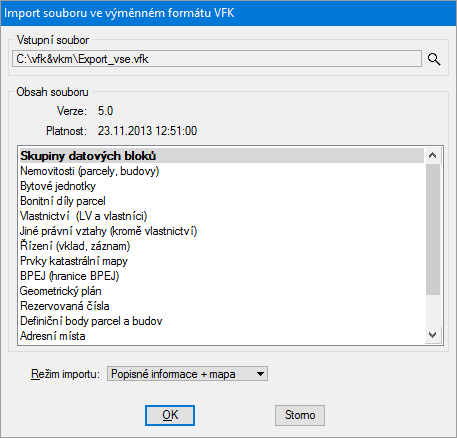
\includegraphics[height=9cm]{./pictures/gisoft.png}
      \caption{Ukázka načtení VFK dat (zdroj:
\href{http://www.gisoft.cz/cze/files/Moduly/import-vfk.png}{gisoft.cz})}
      \label{fig:topol}
  \end{figure}
%zdroj: http://www.gisoft.cz/Moduly/ImportVFK
%obrazek: http://www.gisoft.cz/cze/files/Moduly/import-vfk.png
\subsection{Spirit VFK}
Samospustitelná desktopová aplikace určená pro převod dat katastru nemovitostí do libovolné geodatabáze ESRI. Do geodatabáze jsou importovány tabulky, relace a ostatní databázové objekty \zk{ISKN}. Výslednou databázi jde použít pro analytickou práci na datech kastartu nemovitostí nebo v aplikačních nadstavbách \textit{Spirit KN} a \textit{Spirit Portál} -- KN. Produkt je od společnosti GEOREAL s.r.o. a je zpoplatněný. Po krátké registraci je možné vyzkoušet 30-ti denní Trial verzi \footnote{http://mapy.georeal.cz/trialreg/}.\cite{spirit_vfk}
%zdroj: http://www.georeal.cz/cz/spirit-desktop/spirit-vfk
\subsection{TopoL xT}
TopoL xT je zpoplatněný software od společnosti TopoL. Je to obecný geografický systém určený pro přípravu, správu a analýzu geografických dat. Soubory výměnného formátu katastru nemovitostí - VFK jsou jedním z podporovaných formátu pomocí importu. Pro vyzkoušení je k dispozici demonstrační verze\footnote{http://www.topol.eu/files/download/topol/100/setup.exe}, ve které je omezený počet objektů, omezená velikost rastru a nelze tisknout v měřítku.\citep{topol}

\begin{figure}[H]
	 \centering
      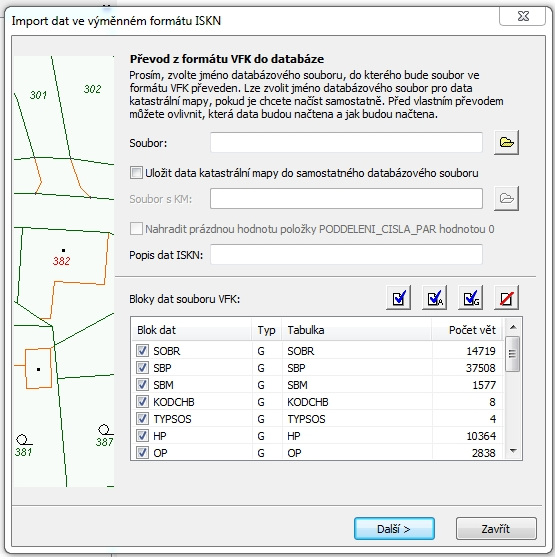
\includegraphics[height=9cm]{./pictures/topol.png}
      \caption{Ukázka importu VFK dat v programu TopoL xT (zdroj:vlastní)}
      \label{fig:topol}
  \end{figure}
%http://www.topol.eu/articles/software#topol-xt
\subsection{Kokeš}
Interakční grafický systém Kokeš od firmy GEPRO s.r.o. je zaměřený na obor geodézie a na geoinformační systémy. V systému je možné řešit nejrůznější geodetické i konstrukční výpočty, vytvářet a aktualizovat kresby map, vést popisné údaje k objektům a bodům mapy, digitalizovat grafické podklady. Budování systému po základních a uživatelských funkcích umožňuje postupný vývoj a jednoduché ovládání. \cite{kokes_cvut}

Funkce import VFK umožňuje importovat jednotlivé soubory, kdy vstupem je jeden nebo více souborů VFK (nebo ZIP) a výsledkem jedna databáze SPI a výkresy katastrální mapy, orientační mapy, definičních bodů parcel a definičních bodů budov. %\citep{napoveda_kokes}

\begin{figure}[H]
	 \centering
      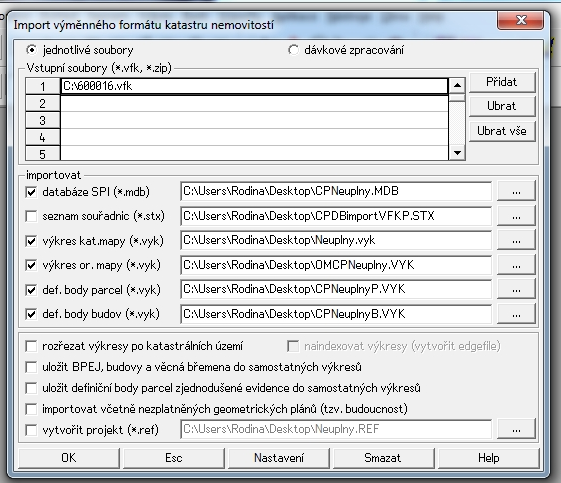
\includegraphics[width=10cm]{./pictures/kokes.png}
      \caption{Ukázka importu VFK dat v programu Kokeš (zdroj:vlastní)}
      \label{fig:kokes}
  \end{figure}
%zdroj: http://geo3.fsv.cvut.cz/~soukup/dip/bukovsky/1.htm, napoveda kokes k funkci import vfk
\subsection{ISKN Studio pro ArcGIS}
Software určený pro import dat formátu \zk{ISKN} do formátu geodatabáze. Pracuje s daty ve formátu NVF a umožňuje jejich zpracování do osobní, souborové a ArcSDE geodatabáze v MS SQL Server či Oracle. K ISKN Studiu jde možné doinstalovat odplněk ISKN View, který slouží k rychlému a jednoduchému vyhledávání v datech ISKN převedených pomocí softwaru ISKN Studio. Jedná se o zpoplatněný software. \cite{arcgis}

\begin{figure}[H]
	 \centering
      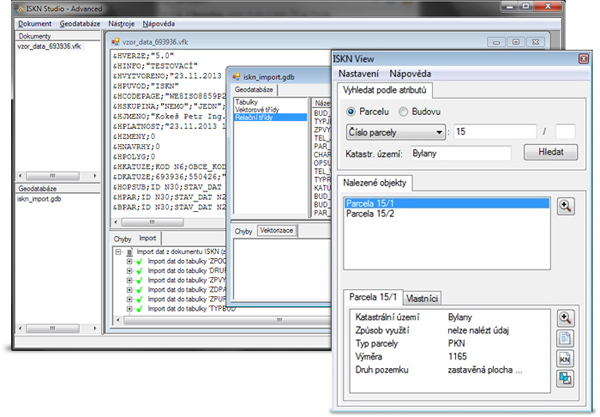
\includegraphics[height=9cm]{./pictures/iskn_studio.jpeg}
      \caption{Ukázka načtení VFK dat v ISKN Studiu (zdroj:
\href{https://www.arcdata.cz/uploads/media/general/0001/01/68f0bfd90cf19d903a57fc8457e1f228a7dd47f4.jpeg}{arcdata.cz})}
      \label{fig:iskn studio}
  \end{figure}
%zdroj:https://www.arcdata.cz/produkty/software-arcdata/import-iskn
%obrázek: https://www.arcdata.cz/uploads/media/general/0001/01/68f0bfd90cf19d903a57fc8457e1f228a7dd47f4.jpeg
\subsection{cadstudio}
V obou případech se jedná o konverzní aplikaci firmy CAD Studio určenou pro zpracování dat \zk{ISKN}.
\begin{itemize}
\item VFK2DB -- import dat do relační databáze Oracle nebo MS SQL Server, samostatný spustitelný program \cite{vfk2db} %http://www.cadstudio.cz/vfk
\item VFK2DWG -- automatický převod souboru či souborů VFK přímo na objekty AutoCADu a nimi svázané databázové tabulky, nadstavba AutoCADu \cite{vfk2dwg}

\begin{figure}[H]
	 \centering
      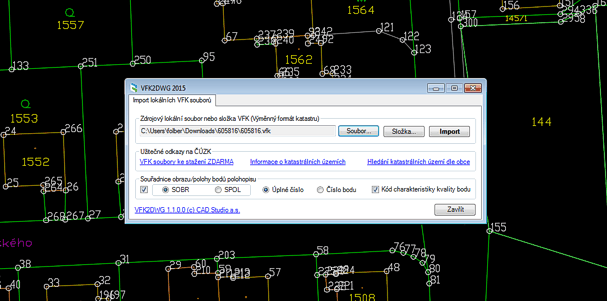
\includegraphics[width=14cm]{./pictures/vfk2dwg.png}
      \caption{Import VFK souborů (zdroj:
\href{http://www.cadstudio.cz/img/vfk2dwg11.gif}{cadstudio.cz})}
      \label{fig:iskn studio}
  \end{figure}
%http://www.cadstudio.cz/vfk2dwg
\end{itemize}
\subsection{knihovna GDAL} 
VFK Driver je součástí knihovny \zk{GDAL} a umožňuje čtení souborů výměnného formátu katastru(VFK). Driver, česky ovladač, slouží obecně k rozšíření funkcionality. Soubor \zk{VFK} je vnímán jako zdroj dat(\verb|OGR datasource|) s žádnou nebo více vrstvami(\verb|OGR layers|). Body jsou ve vrstvách reprezentovány jako \verb|wkbPoints|, linie a hranice jako \verb|wkbLineStrings| a plochy jako \verb|wkbPolygons|. VFK driver si během prvního čtení ukládá data do SQLite databáze, která se vytvoří ve stejném adresáři jako je vfk soubor. Opakované načtení je díky již vytvořené databázi výrazně rychlejší. Výhoda databáze je v snazším a rychlejším přístupu k datům. Dále si může uživatel pomocí proměnných \verb|OGR_VFK_DB_OVERWRITE| a \verb|OGR_VFK_DB_NAME| nastavit jestli bude vytvořená SQL databáze při načtení přepsaná(čtení stále z vfk souboru) a jaký bude název vytvořené databáze. Navíc je tento driver jako jediný z výše zmíněných nástrojů volně dostupný. \cite{vfk_driver}

\begin{figure}[H]
	 \centering
      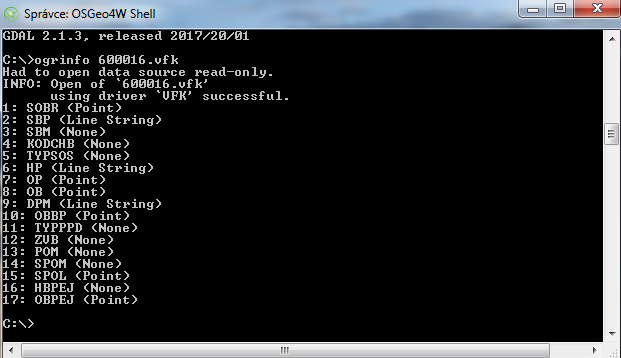
\includegraphics[width=15cm]{./pictures/vfk_driver.png}
      \caption{Ukázka použití VFK driveru (zdroj:vlastní)}
      \label{fig:vfk driver}
  \end{figure}
%zdroj:http://gdal.org/drv_vfk.html
%http://freegis.fsv.cvut.cz/gwiki/VFK_/_GDAL
%http://freegis.fsv.cvut.cz/gwiki/V%C3%BDm%C4%9Bnn%C3%BD_form%C3%A1t_ISKN
%\subsubsection{SQLite driver}
%Ve verzi knihovny \zk{GDAL} 2.1.3 a nižší je nezbytné, aby databáze obsahovala tabulky s upřesněním podoby obsažené geometrie (\verb|geometry columns|) a souřadného systému (\verb|spatial_ref_sys|). Pokud databáze tabulky neobsahuje, SQLite driver nerozezná datový typ vrstvy. Novější verze knihovny si s absencí tabulek dokáže poradit, resp už si tabulky vytvoří sama.
%zdroj: http://gdal.org/drv_sqlite.html

%VFK/QGIS plugin
%http://freegis.fsv.cvut.cz/gwiki/VFK_/_QGIS_plugin
\section{Sestavení geometrie prvků}
K sestavení geometrie prvků dochází až když o ní uživatel požádá. Platí pro verzi knihovny GDAL 2.1 a nižší. Geometrie se sestavuje postupně po blocích dle schématu:
\begin{figure}[H]
	 \centering
      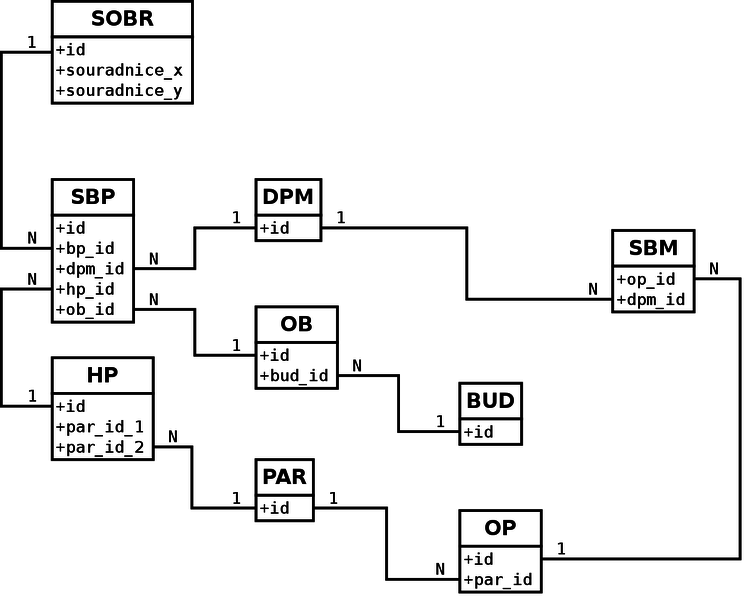
\includegraphics[width=10cm]{./pictures/Vfk-diagram-geom.png}
      \caption{Přehled datových bloků pro sestavení geometrie prvků digitální katastrální mapy (zdroj:
      \href{http://freegis.fsv.cvut.cz/wiki/images/thumb/8/8a/Vfk-diagram-geom.png/744px-Vfk-diagram-geom.png}{freegis.fsv.cvut.cz})}
      \label{fig:vfk diagram geom}
  \end{figure}
Pokud nás tedy zajímá geometrie bloku HP(hranic parcel), dojde k sestavení geometrie i pro všechny předchozí bloky - SOBR(souřadnice obrazu bodů polohopisu) a SBP(spojení bodů polohopisu). Obdobně je to při sestavování bloku OB(obrazy budov) - sestaví se geometrie i pro bloky SBP a SOBR. Zmíněné loky HP a OB jsou podstatné pro tuto práci, protože právě z nich budou pomocí knihovny sestaveny bloky PAR(parcely) a BUD(budovy).
%zdroj: http://freegis.fsv.cvut.cz/gwiki/VFK_/_GDAL